\documentclass[hidelinks, 12pt,letterpaper]{article}
%%%%%%%%%%%%%%%%%%%%%%%%%%%%%%%%%%%%%%%%%%%%%%%%%%%%%%%%%%%%%%%%%%%%%%%%%%%%%%%%%%%%%%%%%%%%%%%%%%%%%%%%%%%%%%%%%%%%%%%%%%%%
\usepackage{amsmath}
%\usepackage{graphicx,fancyheadings}
\usepackage{fancyhdr}
\pagestyle{fancy}
\usepackage{graphics}
\usepackage{amssymb}
\usepackage{verbatim}
\usepackage{setspace}
\usepackage{ulem}

\usepackage{amssymb}
\usepackage{graphicx}
\usepackage{amsmath}
\usepackage{verbatim}
\usepackage{setspace}
\usepackage{ulem}
\usepackage{textpos}
\usepackage{changepage}
\usepackage{url}
\usepackage{hyperref}

\usepackage{color}
\usepackage{xcolor}


%\renewcommand{\sout}[1]{}
%\renewcommand{\bf}{}

\usepackage[round]{natbib}
% \usepackage[backend=biber,style=apa,autocite=inline]{biblatex} \DeclareLanguageMapping{english}{english-apa}
% \addbibresource{./sshrc2023shipping.bib}


%\lhead{} \chead{} \cfoot{}
\renewcommand{\headrulewidth}{0pt}
\renewcommand{\footrulewidth}{0pt}
\renewcommand{\baselinestretch}{1.1}
%\textheight 8in \textwidth 6in \oddsidemargin 0.15in
%\evensidemargin 0in \headheight 14.5pt \headwidth 6in \parskip 4pt

\pagestyle {empty}

\setlength{\topmargin}{0.0cm} \setlength{\headheight}{0cm}
\setlength{\headsep}{0.3cm} \setlength{\topskip}{0cm}
\setlength{\textheight}{22.5cm} \setlength{\textwidth}{16.6cm}
\setlength{\oddsidemargin}{0cm} \setlength{\evensidemargin}{0cm}
\setlength{\footskip}{0.5cm}
\newcommand{\indep}{\perp \!\!\! \perp}


\newcommand{\Red}{\color{red}}
\newcommand{\Blue}{\color{blue}}
\newcommand{\ve}{\varepsilon}

\def\bs{\boldsymbol}

%\setlength{\topmargin}{-0.2cm} \setlength{\headheight}{0cm}
%\setlength{\headsep}{0.3cm} \setlength{\topskip}{0cm}
%\setlength{\textheight}{22cm} \setlength{\textwidth}{16.2cm}
%\setlength{\oddsidemargin}{0cm} \setlength{\evensidemargin}{0cm}
%\setlength{\footskip}{1cm}

\usepackage[letterpaper]{geometry}

\usepackage{graphicx}
\graphicspath{{../images/shared/}}


 \rhead{Hiroyuki Kasahara \hspace{-1.7cm} }
 %\lfoot{}
 \cfoot{\thepage \hspace{-2cm}}



%\setcounter{page}{10}

\begin{document}
\bibliographystyle{asa}

% Challenge—The aim and importance of the endeavour (40\%):
% \begin{itemize}
%   \item originality, significance and expected contribution to knowledge;
%   \item appropriateness of the literature review;
%   \item appropriateness of the theoretical approach or framework;
%   \item appropriateness of the methods/approach;
%   \item quality of training and mentoring to be provided to students, emerging scholars and other highly qualified personnel, and opportunities for them to contribute; and
%   \item potential for the project results to have influence and impact within and/or beyond the social sciences and humanities research community.
% \end{itemize}

% Feasibility—The plan to achieve excellence (20\%):
% \begin{itemize}
%   \item appropriateness of the proposed timeline, and probability that the objectives will be met;
% \end{itemize}

\begin{center}
\textbf{Detailed Description of Proposed Research: }\vspace{-0.25cm}
\end{center}

\noindent \textbf{Project: Quantifying the response of maritime shipping CO$_2$ emissions to economic shocks}
\smallskip

\noindent \textbf{Objective:} There are three goals. First, we quantify a change in the worldwide CO$_2$ emissions from maritime shipping before and during the COVID pandemic. Second, we examine a source of a change in the worldwide CO$_2$ emissions from maritime shipping during the COVID pandemic in terms of a change in different bilateral trade volumes and provide a decomposition analysis. 
Third, we estimate the heterogenous elasticities of CO$_2$ emissions from maritime shipping with respect to international trade using the COVID pandemic demand shock as a source of significant variation, which may be used for conducting a counterfactual analysis of future change in international trade on the worldwide CO$_2$ emissions.   \smallskip

\noindent \textbf{Context:} 
Global trade is intricately linked with maritime shipping, which carries over 80\% of the volume of all traded goods and around 70\% of their value \citep{unctad2017review}.
% The importance of the shipping industry has become particularly apparent in recent years as disruptions ranging from the blockage of the Suez Canal to widespread COVID-related port slowdowns have snarled supply chains world-wide.
At the same time, maritime ships contribute about 3\% of global CO$_2$ emissions, roughly equal to the total emissions of Germany \citep*{faber2020fourth}. These emissions lie outside the scope of national emissions tallies, and fall instead under the jurisdiction the International Maritime Organization (IMO), which has set a target of a 50\% reduction by 2050. %\textcolor{blue}{mention difficulty of decarbonization?}
The stringency of abatement actions required to meet this goal clearly depends on how trade will evolve over the coming decades. A continuation of the trend of increasing trade would make this goal much more difficult to hit. Faced with this uncertainty, the IMO and its consituent countries are developing and implementing policies to reduce shipping emissions, with new efficiency regulations being phased in this year. 
 

The trade volumes substantially fluctuated during the COVID pandemic, where  world merchandise trade decreased by more than 10 percent in the first three months of COVID pandemic  and then slowly recovered over next two years \citep{oecd21}. %Furthermore, the extent to which trade decreased differ across countries and industries.  
In this project, we measure a change in the worldwide CO$_2$ emissions before and during the COVID pandemic using the detailed high-frequency satellite data of ships' movements and analyze the source of a change in  in the worldwide CO$_2$ emission, i.e. a change in bilateral trade volumes across different bilateral relationships as well as across different traded products. Furthermore, by exploiting a large variation in international shipping that resulted from the COVID pandemic, we estimate the elasticity of of CO$_2$ emissions from maritime shipping with respect to international trade, and  quantitatively examine how a change in trade volumes affects the CO$_2$ emission from maritime shipping to inform policy makers.  %We then use the estimated elasticities to compute how a change in trade volumes before and during/after the COVID pandemic led to a change in CO$_2$ emission from maritime shipping across different country pairs, as well as, by aggregate, in the entire world. 

Quantifying this elasticity of CO$_2$ emissions with respect to trade volumes is important for predicting how an increase in international trade affects CO$_2$ emissions in future. Yet, it is challenging for a number of reasons. A ship's fuel consumption depends on various factors, including its size and age (newer and larger ships tend to be more efficient) and the existing fleet is extremely heterogeneous. As an illustration, \autoref{fig:distribution} shows the existing fleet size distribution measured by deadweight tonnage (DWT) for bulk carriers below 100,000 DWT in size (this excludes the largest classes up to just over 400,000 DWT). \textcolor{blue}{Is this a good figure to include? Is it better to use MRV emissions plots instead?}  Because ship sizes are related to types of products shipped as well as port infrastructures, different bilateral trade relationships involves different sizes of ships  and hence  fuel efficiency, leading to heterogenous trade elasticity across different country pairs.  Furthermore, fuel consumption per tonnage depends roughly cubicly on speed, meaning that the short run elasticity of emissions to demand may be quite large and may fluctuate over time as fuel cost or other factors changes. Finally, the presence of trade imbalance leads to ship travels without cargo, making it complicated to estimate the relationship between fuel consumption and trade volumes from the data on ship movements.
% As such, ships adapt differently and which ships change speed or idle is important for determining overall emissions.  


\begin{figure}[h]
  \centering
  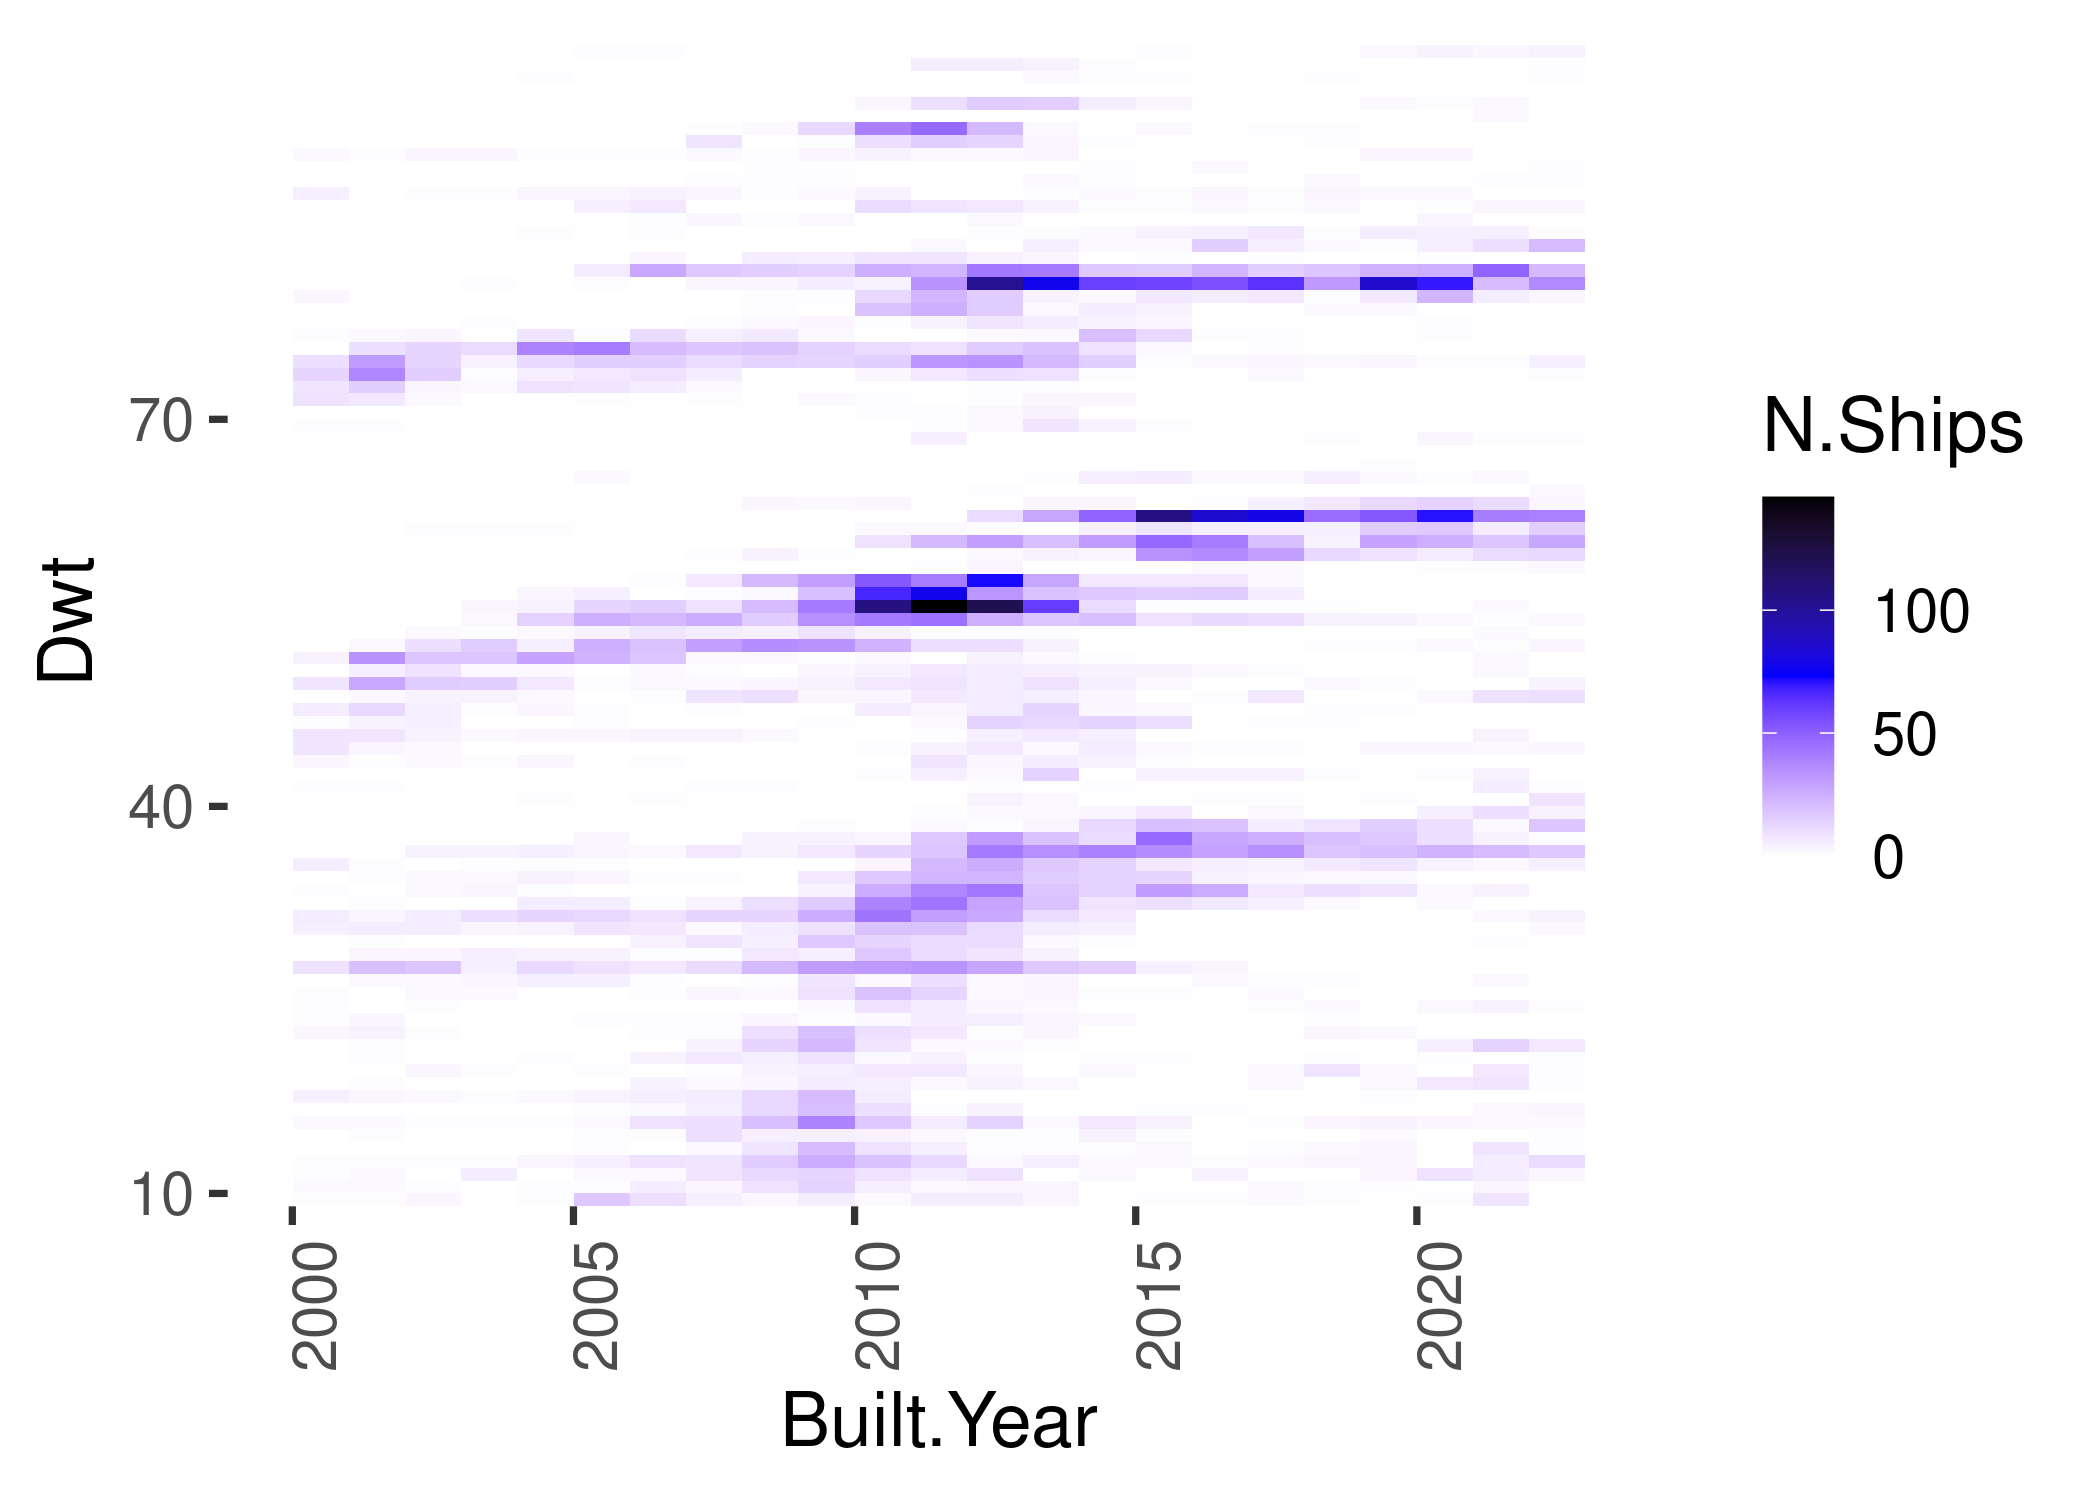
\includegraphics[width = 0.75\textwidth]{WFR_Bulkers_Exploration_Size_Built_heatmap.png}
  \caption{Number of new ships by size (Dwt) and built year \textcolor{blue}{fix labels}
}
  \label{fig:distribution}
\end{figure}

%We use  the detailed high-frequency satellite data of ships' movements merged with the data on ship characteristics as well as the data on annual fuel consumption for EU ships to estimate how fuel efficiency depends on age, speed, size, the level of draft (which measures the capacity utilizations), and other ship characteristics. 

 
 
%
%The three largest sectors of maritime shipping, jointly accounting for over half of maritime emissions, are containerships, bulk carriers, and tankers. These ships transport, respectively,  containerized goods (often manufactured goods), dry bulk goods (e.g. coal, ores, grains), and bulk liquids (primarily oil). As such, they contribute to diverse links of the overall supply chain and are impacted differently by fluctuations in trade. Furthermore, each sector has distinct market characteristics. For example, containerships typically operate with fixed routes and schedules, while bulk carriers tend to operate much more flexibly. Ownership structures reflect these differences as well, with the containership sector being highly concentrated and the bulk carrier sector highly \textit{un}concentrated.
%
%Despite their differences, the various sectors share some common mechanisms by which they adjust to demand. Because new ships cost tens to hundreds of millions of dollars, last for over 25 years, and take two to five years to build, adjustments in fleet capacity are slow to occur. On shorter time horizons, shipping supply adjusts to changing levels of demand primarily through a combination of changing travel speed and temporarily idling ships, though quantifying these adjustments is an active area of research (see \citet*{adland2018dynamic, ollila2022effect,assmann2015missing}). 

%The IMO has introduced three separate emissions regulations. The first, implemented in 2013, is a minimum efficiency requirement for new ships, with stringency increasing over time and future levels yet to be determined. As of the beginning of 2023, a similar regulation now applies to all existing ships and an additional regulation has be added that requires operational efficiency of each ship to be continuously improved moving forward. Uncertainty surrounding these regulations, as well as future technological developments has led to reduced new ship building activity in the past years. With a diminished extrinsic margin for adjustment in addition to the already slow natural fleet development, this places further importance on quantifying the intrinsic margin for predicting the path of shipping emissions.

The most extensive existing literature regarding shipping emissions comes from the IMO itself, in cooperation with a handful of related industry organizations. In particular, the Fourth IMO GHG Study 2020 \citep{faber2020fourth} details both bottom-up and top-down methodologies for calculating emissions. Their bottom-up approach relies on high frequency tracking data and has been developed and employed by various authors (e.g. \citet{olmer2017greenhouse, johansson2017global, jalkanen2009modelling, van2018spatially}). All ships are equipped with automatic identification system (AIS) transceivers which transmit information about the location and speed of each ship every few minutes. In order to estimate emissions, this information is combined with ship fuel consumption ratings and aggregated.

With regards to relating trade to shipping activity, \citet{brancaccio2018impact} explore the elasticity of trade with respect to ship fuel costs. Our work will be some of the first to seriously explore the relationship in the opposite direction - from trade to emissions. To the best of our knowledge, our work will be the first to utilize actual reported emissions to empirically estimate ship efficiencies on a large scale, which allows for more of the previously mentioned channels to be captured. In addition, our approach is novel in its use of machine learning to extrapolate efficiencies for ships without reported emissions. Furthermore, we are not aware of any literature yet that exploits the large variation in shipping activity due to COVID to explore emissions. With these contributions, we hope to provide important quantitative estimates to help inform policy makers in assessing the effectiveness of emissions regulations and setting their stringency levels going forward.


\smallskip

\noindent \textbf{Methodology:}  We first estimate how ship's fuel consumption efficiency  is determined by ship's speed, location, draft, and ship's observed characteristics and compute the  high-frequency disaggregated emissions estimates for each ship's trip  between two ports. This first stage relies on three key datasets that we have obtained: (i) AIS tracking data, (ii)  the World Fleet Register, and (iii) the MRV data that reports individual emissions.

We have obtained hourly AIS tracking data for the entire fleets of bulk carriers and containerships from the beginning of 2019 to the end of 2021. This includes information on speed, location, and draft (the vertical distance between the waterline and the bottom of the hull), which can be used to determine whether a ship is carrying cargo or not. This data is then matched to the World Fleet Register from Clarksons Research, which is a virtually complete listing of all large merchant ships. It includes basic  information on each ship, including built year, size, and type, and for many ships includes highly detailed technical characteristics such as hull dimensions, engine power, propeller details, etcetera. Finally, this can be further linked to publicly available data collected through the European Union's Monitoring, Reporting, and Verification (MRV) regulation, which provides annual fuel consumption and emissions for trips into and out of the EU (EU trips, hereafter). This data begins in 2018 and naturally includes only ships with portcalls in the European Union in a given year.

Our methodology of estimating the fuel efficiency builds on that of the IMO as detailed in \citet{faber2020fourth} and follows closely the data cleaning and matching procedures described therein. However, whereas they use \textit{nominal} fuel consumption values corresponding to rather coarse ship size- and age-bins, we propose to empirically estimate more ship-specific fuel efficiencies. In particular, we use actual fuel consumption data  from the MVR data while  \citet{faber2020fourth} does not use any fuel consumption data  by themselves--- rather, fuel consumption is computed using pre-determined formula based on prior experiments on specific types of ships. By using actual fuel consumption data, we hope to better estimate how fuel consumption is determined under actual operating conditions. 


Our procedure consists of four steps: First, we estimate fuel efficiency is determined by operating conditions (speed, draft) and ship characteristics (age, deadweight tonnage etc.) using the data on EU trips reporting in the MRV dataset. 
Then, we extrapolate these efficiencies to non-reporting ships, i.e., ships that never stopped at any EU ports, based on operating condition and ship characteristics. Given ship efficiencies, we can calculate a high frequency emissions estimate for each ship. Finally, these estimates can be aggregated at any desired level. To our knowledge, this will be the first work to employ the MRV data to estimate fuel efficiency. \citet{uge2020estimation} also link MRV data with AIS data, but they use it in the opposite sense, namely to validate reported emissions in the MRV.

To date, we have estimated fuel efficiencies using this procedure for bulk carriers. We have further constructed a predictive model for efficiency extrapolation, regressing fuel efficiency on a set of ship characteristics (using logs of all variables) as well as built-year fixed effects.
 \begin{equation}
 \log\left(
     \frac{fuel~consumption}{Dwt \cdot \sum_{x \in X}  \cdot s_x^2 \cdot x}
 \right)_{it}
         = \delta age_{it} + \boldsymbol{\beta}f(Z_i) + \varepsilon_{it},
 \end{equation}
 where $Z_i$ is a vector of ship's characteristics and $f(\cdot)$ is an unknown function, which we use semi-parametric sieve method using B-splines as well as machine learning tools (e.g., random forest, XGboost, deep neural network) to estimate.
The coefficients for the built-year fixed effects for our preliminary estimation based on log-linear specification are plotted in \autoref{fig:efficiency} and indicate that efficiency after controlling for size is surprisingly flat for ships built before roughly 2013, after which efficiency improved. This agrees qualitatively with the analysis of evolution of new ship efficiency from \citet{faber2015historical} (see Figure 15). The current specification does not include the effects of laden status or weather but we plan to include  the draft level as well as wind and wave speeds using detailed weather data like that used by \citet{brancaccio2020geography}.  %As noted by \citet{olmer2017greenhouse}, details such as the engine power curve (how fuel consumption varies away from design speed), hull-roughening, and hull-fouling are hard to predict or attribute. 

A limitation of our proposed approach is that the fuel consumption data is annual and there may be significant error in calculating the travel work over such a long time period. On the other hand, the advantage of this approach over that used by \citet{faber2020fourth} is that it relies less on theoretical assumptions. We plan to compare our CO$_2$ emission estimate with the estimate from \citet{faber2020fourth}. %Our estimates would incorporate these effects at the average level of observed ships

After estimating fuel consumption for each ship's trip, we estimate the worldwide CO$_2$ emission within each month of the years from 2017 to 2022 by aggregating fuel consumptions from all trips. Furthermore, we identify fuel consumption at more disaggregated level, i.e., the fuel consumption associated with maritime shipping from port A to port B by aggregating all trips taken from port A to port B in each month.  Then, by aggregating all ports within each country for source and destination country, we estimate the monthly CO$_2$ emission associated with maritime shipping from country A to country B. 
This allows us to analyze the source of  a change in the worldwide CO$_2$ emission by decomposing it as the sum of a change in bilateral trade flows across different countries and direction. 
Here, we take into account of imbalance in trade volumes by identifying ship loading and unloading at each port using the high frequency data on the level of draft, where 42\% of ships are found to be travelling without cargo \citep{brancaccio2020geography}.
  
Because the MRV data encompasses only trips in and out of the EU, in order to estimate fuel efficiency, we must first detect trips from the tracking data and identify those that involve a portcall in the EU. We detect stops based on a ship speed threshold and a location near to land and denote a trip  as a trip between any two stops. In order to ensure the accuracy of our data, we then use data only for ship-year observations for which the total distance of detected trips to/from the EU agrees closely with the distance reported in the MRV data. With this travel history constructed, we calculate a proxy for the travel work performed by a ship in a given year as the sum of its speed squared multiplied by the distance travelled between every pair of observations in the AIS data. The fuel efficiency is then calculated as the reported annual fuel consumption divided by the inferred annual travel work.
.

%To date, we have estimated efficiencies using this procedure for bulk carriers. We have further constructed a simple linear predictive model for efficiency extrapolation, regressing fuel efficiency on a set of ship characteristics (using logs of all variables) as well as built-year fixed effects.
% \begin{equation}
% \log\left(
%     \frac{fuel~consumption}{Dwt \cdot \sum_{x \in X}  \cdot s_x^2 \cdot x}
% \right)_{it}
%         = \delta age_{it} + \boldsymbol{\beta}log(Z_i) + \varepsilon_{it}
% \end{equation}
%The coefficients for the built-year fixed effects are plotted in \autoref{fig:efficiency} and indicate that efficiency after controlling for size is surprisingly flat for ships built before roughly 2013, after which efficiency improved. This agrees qualitatively with the analysis of evolution of new ship efficiency from \citet{faber2015historical} (see Figure 15).

\begin{figure}[h]
  \centering
  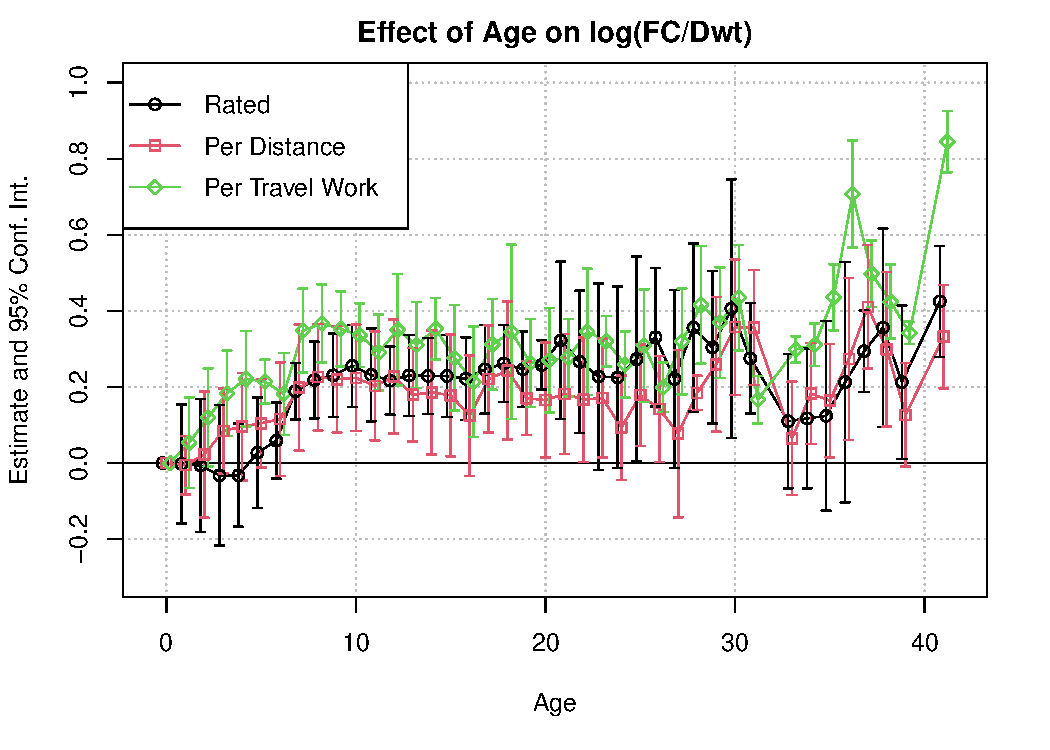
\includegraphics[width = 0.75\textwidth]{Efficiency_Regression_Size_Age_Coeffs_3.pdf}
  \caption{\textcolor{blue}{update, tidy, fix labels}}
  \label{fig:efficiency}
\end{figure}

Our next step is to assess the quality of extrapolation in a more systematic manner using cross-validation on randomly selected training and testing subsets. We are also developing an alternative, more flexible neural network model for efficiency extrapolition, and will compare its performance to the simple linear model. Finally, this exercise will be repeated for containerships.

% Trade
%% Data
COVID variation
\textbf{Trade data} Bilateral trade data from...

\textbf{Method of linking to emissions to trade}
Begin with global, then incorporate geographical variation


\pagebreak
Potential data purchases:
\begin{itemize}
  \item expand time series of AIS tracking data beyond 2021
  \item AIS tracking data for tankers
  \item bilateral trade
\end{itemize}

\pagebreak

% \printbibliography[heading = subbibliography]
\singlespace{
\bibliography{sshrc2023shipping}
}



\end{document}
